% GreenPEFT paper draft.
% Build:  pdflatex main && bibtex main && pdflatex main && pdflatex main
% Every number is traceable: a "% [src: ...]" comment beside it names the file it comes from.
% Figures and paper/data/*.csv are regenerated by:  python paper/scripts/build_paper_assets.py
\documentclass[conference]{IEEEtran}

\usepackage[T1]{fontenc}
\usepackage{graphicx}
\usepackage{booktabs}
\usepackage{multirow}
\usepackage{amsmath,amssymb}
\usepackage{url}
\usepackage[hidelinks]{hyperref}
\usepackage{cite}

\newcommand{\COtwo}{CO\textsubscript{2}e}
\graphicspath{{figures/}}

\begin{document}

\title{GreenPEFT: A Multi-Objective Green AI Decision Support Framework for Sustainable
Parameter-Efficient Fine-Tuning}

\author{\IEEEauthorblockN{Ashraful Islam Tanzil}
\IEEEauthorblockA{United International University}}

\maketitle

% =====================================================================================
\begin{abstract}
Parameter-efficient fine-tuning (PEFT) lowers the cost of adapting large language models,
but practitioners still have to choose among methods and model scales without knowing in
advance what a configuration will cost in memory, energy and time. We present GreenPEFT, a
decision-support framework built on a controlled single-GPU benchmark. We fine-tuned four
backbones (0.5B--3.0B parameters) with full fine-tuning, LoRA, QLoRA, LoRA-FA and LISA on
SST-2 on one NVIDIA Tesla T4, measuring accuracy, peak GPU memory, GPU energy and runtime.
Operational \COtwo{} was then estimated from measured energy with a fixed carbon-intensity
factor. A measurement audit found that the benchmark's two measurement passes are not
independent and that one pass recorded the GPU idle-power floor instead of training power; we
therefore base all energy results on the single valid pass of 41 completed configurations.
On these data we fit four Ridge surrogates that predict accuracy, peak memory, energy and
runtime from metadata available before a run starts, and we evaluate them under both
interpolation and leave-one-scale-out protocols. Energy is predicted well even at a held-out
scale ($R^2=0.90$, MAPE $10.6\%$). Memory, runtime and accuracy interpolate well but
extrapolate weakly ($R^2$ 0.08--0.59), so the surrogate as a whole is rated preliminary. The
predictions feed a constraint filter, a four-objective Pareto frontier and configurable
preference profiles, and every recommendation is labelled with its evidence scope. The data,
model and command-line tool are released with DOIs.
\end{abstract}

\begin{IEEEkeywords}
Green AI, parameter-efficient fine-tuning, energy measurement, surrogate modelling,
multi-objective decision support, LoRA, QLoRA
\end{IEEEkeywords}

% =====================================================================================
\section{Introduction}

Training and adapting neural language models consumes electricity, and the resulting
emissions have become part of how the field evaluates its own methods
\cite{strubell2019energy,schwartz2020greenai,henderson2020reporting,patterson2021carbon}.
Schwartz et al.\ argued that efficiency should be reported next to accuracy, not left
implicit \cite{schwartz2020greenai}. For most practitioners the relevant workload is
fine-tuning a pre-trained model on modest hardware, not pretraining one.

Parameter-efficient fine-tuning (PEFT) is the usual response to that constraint. Low-rank
adaptation (LoRA) trains small rank-decomposition matrices while freezing the base weights
\cite{hu2022lora}; QLoRA adds a 4-bit quantized base model \cite{dettmers2023qlora}; LoRA-FA
freezes one of the two low-rank factors \cite{zhang2023lorafa}; and LISA samples a small set
of full layers to update at each period \cite{pan2024lisa}. Surveys catalogue many more
variants \cite{han2024peftsurvey}. These methods save different resources. A method that
saves memory need not save energy, and one that saves energy may take longer. A practitioner
with a fixed GPU and an energy or time budget therefore faces a multi-objective choice, and
usually has no measurement of the options before running them.

This paper asks how measured PEFT performance and resource cost can be modelled and used to
support that choice under practical constraints. We do not try to identify a universally
best or greenest method. We address three research questions:

\begin{itemize}
\item \textbf{RQ1.} How do PEFT strategies differ in task performance and resource
consumption on a constrained single GPU?
\item \textbf{RQ2.} Can pre-run configuration features predict accuracy, GPU memory, energy
and training time?
\item \textbf{RQ3.} Can those predictions support constraint-aware selection of
resource-conscious configurations?
\end{itemize}

Our contributions are:
(i) a controlled empirical PEFT dataset with a documented measurement-validity audit that
identifies a duplicate-pass structure and an idle-floor telemetry defect;
(ii) a pre-run surrogate evaluated under grouped interpolation and leave-one-scale-out
protocols, with status set by the weaker protocol;
(iii) a decision-support layer that combines surrogate predictions, user constraints, a
Pareto frontier and preference profiles, and labels each recommendation with its evidence
scope; and
(iv) released data and model artifacts with DOIs \cite{tanzil2026data,tanzil2026model}.

% =====================================================================================
\section{Related Work}

\textbf{Parameter-efficient fine-tuning.} Adapter layers \cite{houlsby2019adapters} and
low-rank adaptation \cite{hu2022lora} established that a small number of trainable
parameters can approach full fine-tuning quality. QLoRA reduces memory further through 4-bit
NormalFloat quantization of the frozen base model and double quantization
\cite{dettmers2023qlora}. LoRA-FA freezes the projection-down matrix of each adapter to
reduce activation memory \cite{zhang2023lorafa}. LISA keeps full-parameter updates but
restricts them to randomly sampled layers \cite{pan2024lisa}. Han et al.\ survey the wider
family \cite{han2024peftsurvey}. These works mostly report accuracy together with memory or
trainable-parameter counts. Energy and runtime under a common hardware budget are reported
less often, and rarely for several methods at once.

\textbf{Green AI and energy accounting.} Strubell et al.\ quantified the energy and emissions
of training NLP models \cite{strubell2019energy}. Later work proposed systematic reporting
frameworks \cite{henderson2020reporting}, emission calculators \cite{lacoste2019quantifying}
and analyses of large-scale training \cite{patterson2021carbon}. Tools such as CodeCarbon
estimate emissions as measured energy multiplied by the carbon intensity of the electricity
supply \cite{codecarbon2024}. GPU power is commonly read through NVIDIA's management library
(NVML) \cite{nvml}. We follow the same accounting: energy is measured, and \COtwo{} is
derived from it.

\textbf{Positioning.} Prior PEFT studies compare methods. Prior Green AI studies measure or
report footprints. This work connects the two. It treats the measured cost of PEFT
configurations as data, fits a model that predicts that cost before a run, and uses the
predictions for constrained selection. The study is deliberately narrow, covering one task,
one GPU and four model scales, and the claims below are limited to that scope.

% =====================================================================================
\section{Dataset and Experimental Methodology}

\begin{figure*}[t]
\centering
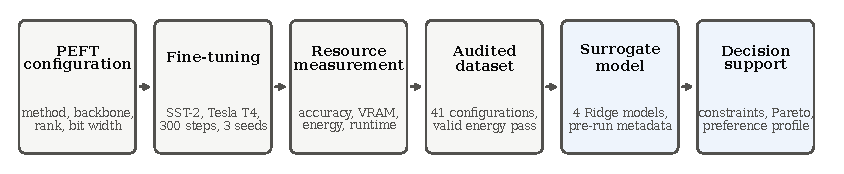
\includegraphics[width=\textwidth]{fig1_pipeline.pdf}
\caption{GreenPEFT pipeline. Configurations are fine-tuned and measured. The audited
measurements train a surrogate on pre-run metadata, and the surrogate's predictions drive
constraint-aware decision support.}
\label{fig:pipeline}
\end{figure*}

Fig.~\ref{fig:pipeline} summarises the pipeline. Table~\ref{tab:setup} lists the setup.

\subsection{Benchmark}

All runs used one NVIDIA Tesla T4 with a 15.6\,GB memory budget on the Kaggle platform. % [src: results/canonical_benchmark/manifest.json]
The task was binary sentiment classification on SST-2 \cite{socher2013sst,wang2018glue},
evaluated on the 872-example validation split. % [src: raw_runs/*.json performance.n_eval]
Each run trained for 300 optimizer steps with batch size 8, gradient accumulation 2, maximum
sequence length 128, dynamic padding and fp16 compute, under seeds 13, 42 and 2024. % [src: raw_runs/*.json budget; manifest.json seeds]
The backbones were Qwen2.5-0.5B, TinyLlama-1.1B-Chat-v1.0, Qwen2.5-1.5B and Qwen2.5-3B
\cite{qwen2024qwen25,zhang2024tinyllama}. % [src: manifest.json backbones]
LoRA, QLoRA and LoRA-FA used rank 16, $\alpha=32$ and dropout 0.05 with learning rate
$2\times10^{-4}$. QLoRA used NF4 with double quantization, and LoRA-FA froze the $A$ matrix.
LISA used learning rate $5\times10^{-5}$, layer-sampling probability 0.25 and resampling
every 20 steps. Full fine-tuning used $2\times10^{-5}$. % [src: results/canonical_benchmark/configs/methods/*.yaml]
The software stack was PyTorch 2.10.0 (CUDA 12.8), Transformers 5.17.0 and PEFT 0.21.0
\cite{wolf2020transformers,mangrulkar2022peft}. % [src: notebooks/green_peft_benchmark_execution.ipynb outputs]

\begin{table}[t]
\centering
\caption{Experimental setup}
\label{tab:setup}
\small
\begin{tabular}{@{}ll@{}}
\toprule
Task & SST-2 binary classification (872 eval.) \\
GPU & 1$\times$ NVIDIA Tesla T4, 15.6\,GB budget \\
Backbones & Qwen2.5-0.5B, TinyLlama-1.1B, \\
          & Qwen2.5-1.5B, Qwen2.5-3B \\
Methods & Full FT, LoRA, QLoRA, LoRA-FA, LISA \\
Budget & 300 steps, batch 8, grad.\ accum.\ 2, len.\ 128 \\
Seeds & 13, 42, 2024 \\
Measured & accuracy, peak GPU memory, \\
         & GPU energy, wall-clock time \\
Derived & \COtwo{} $=$ energy $\times$ 0.65\,kg\,kWh$^{-1}$ \\
\bottomrule
\end{tabular}
\end{table}

\subsection{Measurements}

Accuracy, peak GPU memory, GPU energy and wall-clock time were measured for each run. GPU
energy was integrated from NVML board-power samples at roughly 5\,Hz \cite{nvml}. % [src: raw_runs/lora_tiny_classification_seed13.json: 531 samples / 108.6 s]
Operational \COtwo{} was estimated from measured energy using a fixed carbon-intensity factor
of 0.65\,kgCO$_2$e/kWh. It is a derived quantity, never modelled separately and never
measured directly. % [src: manifest.json grid_carbon_kg_per_kwh; DATA_METHODOLOGY.md 4.2]
In the dataset, the ratio of recorded carbon to energy lies between 0.649988 and 0.650015.
\COtwo{} is therefore a linear rescaling of energy and is reported only as a table column.

\textbf{Scope.} Configurations that exceeded the 15.6\,GB VRAM budget are outside the study's
scope. The models therefore predict cost \emph{given} that a configuration runs. % [src: DATA_METHODOLOGY.md 2 "Scope filter"; model_metadata.json scope]
The study covers 41 completed configurations, defined as method, backbone and seed
combinations. % [src: paper/data/audit_numbers.json n_configurations]
It does not cover a complete grid of methods, backbones and seeds.

\subsection{Data sources and harmonization}

Four candidate sources were collected and mapped onto a common schema with provenance
columns. The result is a harmonized table of 477 rows and 46 columns. % [src: paper/data/audit_numbers.json dataset_shape]
Each row carries an explicit analysis role.
(i) The primary source is our own fine-tuning sweep, which supplies the 82
\texttt{surrogate\_train} rows (41 configurations $\times$ 2 measurement passes).
(ii) The Open LLM-Perf inference leaderboard supplies 369 \texttt{scale\_reference} rows.
(iii) Published pretraining-energy figures for frontier models supply 26
\texttt{context\_only} rows. % [src: DATA_METHODOLOGY.md 7]
Sources (ii) and (iii) measure inference or pretraining, which are different quantities from
fine-tuning cost. They are kept only as scale context and are never used to fit the
surrogate. A fourth source was rejected on three grounds: its model names match no real
release, its efficiency metrics are unitless, and it has no parameter-count column. % [src: DATA_METHODOLOGY.md 1.4]

Deduplication used the run identifier alone. Deduplicating on configuration columns would
have collapsed seed replicates. Missingness in the merged table is structural: whole
columns are absent for whole sources. Outcome metrics were therefore never imputed across
sources. Within the primary sweep, every retained run reported every metric. % [src: DATA_METHODOLOGY.md 2, 3, 5]

\subsection{Measurement-validity audit}

Five audits were run before modelling: exact duplicates, collinear targets, physical
plausibility bounds, seed-replicate outliers (median-absolute-deviation $z>3.5$, flagged but
retained) and the measurement regime. % [src: DATA_METHODOLOGY.md 4]
The last audit changed the analysis.

The 82 training rows are 41 configurations measured twice, not 82 independent runs.
Accuracy is identical across the two passes, so the second pass adds no information for that
target. Converting each pass's energy and runtime into implied average power separates the
two passes clearly. The original pass averages 59.9\,W (range 38.4--65.6\,W), which is
physically consistent with a 70\,W-TDP T4 under load. The re-measured pass reports
$9.97\pm0.10$\,W across a sixfold range of model sizes, which matches the NVML idle floor. % [src: paper/data/audit_numbers.json implied_power_*]
Re-measured energy is therefore flagged \texttt{energy\_measurement\_valid}$\,=0$ and excluded
from every energy analysis, so energy rests on one valid pass of 41 configurations. Pooling
both passes had inflated the coefficient of variation of energy from 0.509 to 0.936. % [src: paper/data/audit_numbers.json energy_cv_*]
For modelling and reporting, each configuration is collapsed to one canonical row. That row
holds the shared accuracy, the pass mean of peak memory and runtime, and the valid-pass
energy. % [src: analysis/greenpeft_data.py load_canonical_runs]

\subsection{Pre-run features}

The surrogate uses 22 features, all known before a run starts. % [src: models/model_metadata.json features]
The features fall into four groups.
Scale features are the parameter count, its logarithm, parameter count $\times$ bit width and
its logarithm.
Method features are bit width, adapter rank, $\log(1+\text{rank})$, the adapter, quantized and
full-fine-tuning indicators, and adapter capacity.
Trainable-size features are the trainable-parameter percentage, the trainable fraction and
the trainable parameter count.
Memory-physics features are weight bytes, optimizer state, gradient memory, their sum
(a memory proxy) and its ratio to the device budget. The categorical features are method and
architecture family.
Reporting ratios that contain an outcome, for example energy per accuracy point, are kept out
of the feature matrix, and this is checked by an assertion. % [src: AUDIT_REPORT.md 3]

% =====================================================================================
\section{Surrogate Model}

\textbf{Models.} We fit one pipeline per target: accuracy, peak GPU memory, energy and
wall-clock time. Each pipeline applies median imputation and standardization to the 20
numeric features, constant imputation and one-hot encoding to the two categorical features,
and then a Ridge regressor ($\alpha=1$) \cite{pedregosa2011sklearn}. Energy and runtime are
fitted on a log scale and back-transformed. All four models are fitted on the 41 canonical
configurations. Carbon is not modelled. A predicted \COtwo{} value is predicted energy
$\times\,0.65$. % [src: models/model_metadata.json model_classes, training_configs]

\textbf{Validation protocols.} The surrogate is meant to score configurations that have not
been run, so random $k$-fold would overstate its accuracy. We report three grouped protocols,
all recomputed on the 41 canonical configurations. % [src: paper/scripts/build_paper_assets.py]
\begin{itemize}
\item \emph{Pass-grouped} 5-fold \texttt{GroupKFold} on \texttt{config\_id}. This protocol
blocks measurement-pass leakage only. Because \texttt{config\_id} contains the seed, other
seeds of the same cell remain in training. It measures \emph{interpolation within measured
scales}.
\item \emph{Seed-grouped} 5-fold \texttt{GroupKFold} on method $\times$ backbone. All seeds
of a cell are held out together. This is still interpolation, because every scale tier
remains in training.
\item \emph{Leave-one-tier-out}, which holds out one backbone scale at a time. This protocol
measures prediction at an unmeasured scale, which is the surrogate's intended use.
\end{itemize}
We report MAE, RMSE, $R^2$ and MAPE. Measured accuracy spans only 0.086 (0.864--0.950), so
$R^2$ for accuracy is unstable, and accuracy is read by MAPE. % [src: paper/data/audit_numbers.json accuracy_range]

\textbf{Status labels.} Each target receives an internal engineering status. VALIDATED
requires $R^2\ge0.70$ and MAPE $\le15\%$. PRELIMINARY requires $R^2\ge0$ and
MAPE $\le50\%$. These thresholds are a project choice recorded in the validation script, not
an external standard. A target's status is the weakest status across protocols. % [src: surrogate/validate.py THRESHOLDS]

% =====================================================================================
\section{GreenPEFT Decision-Support Framework}

Given user constraints, GreenPEFT proceeds in seven steps. % [src: green_peft_cli/.../recommender.py]
\begin{enumerate}
\item \emph{Candidates.} It enumerates the cross-product of a 14-backbone catalogue and the
five methods, giving 70 candidates. The catalogue includes the four measured backbones and
ten unmeasured ones.
\item \emph{Features.} It builds the same pre-run features used in training.
\item \emph{Prediction.} It predicts the four targets and derives \COtwo{}.
\item \emph{Sanity filter.} It drops physically impossible predictions, namely negative peak
memory or accuracy above 1, which the linear models can produce far outside the measured
range. In the scenarios below, 12 of 70 candidates are dropped at this step. % [src: green-peft CLI text output, scenario A]
\item \emph{Constraint filter.} Predicted peak memory must fit within the user's VRAM budget
with a 10\% safety margin, and optional floors or ceilings on accuracy, carbon and time are
applied.
\item \emph{Pareto frontier.} It marks non-dominated candidates on four objectives: maximise
accuracy and minimise memory, energy and runtime.
\item \emph{Ranking.} It ranks the feasible candidates with a Green Efficiency Index (GEI).
\end{enumerate}
The GEI is
\begin{equation}
\mathrm{GEI} = w_A S_A + w_M S_M + w_E S_E + w_T S_T,
\end{equation}
where each $S$ is a min--max normalised score computed over the feasible candidate set.
Higher is better for accuracy and lower is better for the other three objectives. The tool
normalises predicted \COtwo{}, which is proportional to predicted energy, so its min--max
score equals the energy score. The GEI is relative to the candidate set and is not an
absolute rating. It never decides feasibility; constraints do. The named profiles
$(w_A, w_M, w_E, w_T)$ are \texttt{balanced} (0.35, 0.25, 0.25, 0.15),
\texttt{strict\_carbon} (0.20, 0.20, 0.50, 0.10) and \texttt{high\_accuracy}
(0.60, 0.15, 0.15, 0.10). These weights are configurable project preferences, not scientific
constants. % [src: recommender.py GEI_PROFILES]

Each candidate also receives an evidence scope and a confidence level.
\texttt{MEASURED} (HIGH) means the method $\times$ backbone cell was benchmarked.
\texttt{INTERPOLATED\_SCALE} (MEDIUM) means the candidate lies inside 0.5--3.0B and a seen
family. \texttt{UNSEEN\_FAMILY} and \texttt{OUT\_OF\_RANGE\_SCALE} are both LOW. The tool
attaches error bands derived from the surrogate's own out-of-sample MAPE. For candidates
outside 0.5--3.0B those bands are lower bounds, because leave-one-tier-out only ever held
out tiers \emph{inside} that range. % [src: green_peft/confidence.py; model_metadata.json training_envelope]

% =====================================================================================
\section{Results}

\subsection{RQ1: Measured accuracy and resource cost}

Primary comparisons use only method $\times$ backbone cells in which all three seeds completed
with valid telemetry. There are 13 such cells, covering 39 runs: all five methods at 0.5B;
LISA, LoRA, LoRA-FA and QLoRA at 1.1B; LISA, LoRA-FA and QLoRA at 1.5B; and QLoRA at 3.0B.
The 1.5B LoRA cell has fewer than three seeds and is excluded from the primary figures and
tables. It remains in the surrogate's training data. % [src: paper/data/audit_numbers.json]
Table~\ref{tab:results} and Figs.~\ref{fig:energy}--\ref{fig:vram} report the results.

\begin{table*}[t]
\centering
\caption{Measured results for complete cells (mean $\pm$ SD over three seeds). Energy is from
the valid telemetry pass; peak memory and runtime are averaged over both passes before
aggregation; \COtwo{} is derived as energy $\times$ 0.65\,kg/kWh.}
\label{tab:results}
\small
% [src: paper/data/table2_complete_cells.csv]
\resizebox{\textwidth}{!}{%
\begin{tabular}{@{}llcccccc@{}}
\toprule
Backbone & Method & Accuracy & Peak VRAM (GB) & Energy (Wh) & Runtime (s) & Est.\ \COtwo{} (g) & $n$ \\
\midrule
\multirow{5}{*}{Qwen2.5-0.5B}
 & Full FT & $0.905\pm0.006$ & $11.13\pm0.03$ & $2.39\pm0.01$ & $135.7\pm0.6$ & 1.56 & 3 \\
 & LoRA    & $0.917\pm0.001$ & $4.34\pm0.39$  & $1.22\pm0.07$ & $112.4\pm0.7$ & 0.79 & 3 \\
 & QLoRA   & $0.912\pm0.008$ & $2.76\pm0.50$  & $2.15\pm0.01$ & $171.9\pm0.9$ & 1.40 & 3 \\
 & LoRA-FA & $0.916\pm0.002$ & $4.30\pm0.45$  & $1.30\pm0.00$ & $107.8\pm0.8$ & 0.84 & 3 \\
 & LISA    & $0.887\pm0.022$ & $5.11\pm0.24$  & $1.26\pm0.02$ & $73.8\pm1.3$  & 0.82 & 3 \\
\midrule
\multirow{4}{*}{TinyLlama-1.1B}
 & LoRA    & $0.944\pm0.005$ & $9.43\pm1.13$  & $1.77\pm0.03$ & $107.0\pm1.2$ & 1.15 & 3 \\
 & QLoRA   & $0.938\pm0.004$ & $3.96\pm1.35$  & $2.72\pm0.02$ & $161.7\pm0.8$ & 1.77 & 3 \\
 & LoRA-FA & $0.925\pm0.001$ & $8.38\pm0.65$  & $1.73\pm0.01$ & $102.4\pm0.4$ & 1.12 & 3 \\
 & LISA    & $0.920\pm0.006$ & $10.88\pm0.05$ & $2.09\pm0.02$ & $116.9\pm0.5$ & 1.36 & 3 \\
\midrule
\multirow{3}{*}{Qwen2.5-1.5B}
 & QLoRA   & $0.943\pm0.003$ & $6.42\pm1.98$  & $3.44\pm0.04$ & $200.3\pm1.9$ & 2.23 & 3 \\
 & LoRA-FA & $0.943\pm0.004$ & $12.20\pm1.39$ & $2.16\pm0.06$ & $125.1\pm1.1$ & 1.40 & 3 \\
 & LISA    & $0.938\pm0.005$ & $15.21\pm0.63$ & $2.53\pm0.01$ & $141.0\pm0.8$ & 1.64 & 3 \\
\midrule
Qwen2.5-3B & QLoRA & $0.948\pm0.001$ & $7.14\pm0.00$ & $6.01\pm0.01$ & $336.1\pm1.5$ & 3.91 & 3 \\
\bottomrule
\end{tabular}}
\end{table*}

\begin{figure}[t]
\centering
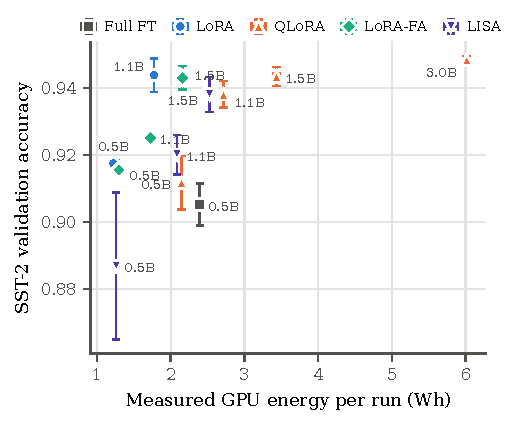
\includegraphics[width=\columnwidth]{fig2_accuracy_energy.pdf}
\caption{Measured accuracy versus GPU energy per run for the 13 complete cells (mean $\pm$ SD
over three seeds). Labels give the backbone size.}
\label{fig:energy}
\end{figure}

\begin{figure}[t]
\centering
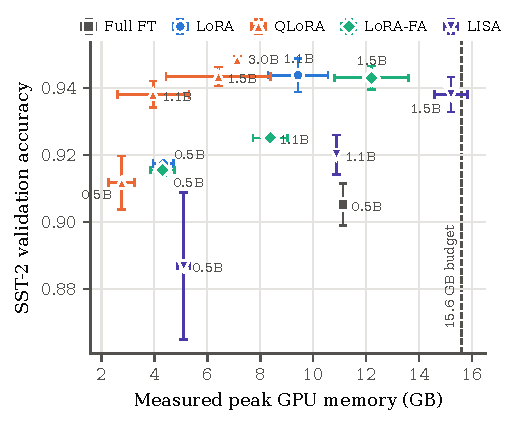
\includegraphics[width=\columnwidth]{fig3_accuracy_vram.pdf}
\caption{Measured accuracy versus peak GPU memory for the 13 complete cells (mean $\pm$ SD
over three seeds). The dashed line marks the 15.6\,GB device budget.}
\label{fig:vram}
\end{figure}

Memory savings and energy savings are different axes. At 0.5B, the only scale where full
fine-tuning is a complete cell, the PEFT methods can be compared with full fine-tuning on
the same backbone. % [src: paper/data/paired_vs_fullft_0p5b.csv]
LoRA reduced energy by 49.0\%, peak memory by 61.0\% and runtime by 17.2\%, with accuracy
1.22 points higher. LoRA-FA gave similar savings (45.7\%, 61.4\%, 20.5\%; $+1.03$ points).
QLoRA gave the largest memory saving (75.2\%) but saved only 10.3\% of energy and took 26.7\%
\emph{longer}, consistent with the extra cost of 4-bit dequantization. LISA ran fastest
(45.6\% less time) and saved 47.4\% of energy, but its accuracy was 1.84 points lower and it
had the largest seed variance of any cell (SD 0.022).
These differences hold for one task, one GPU and one training budget, and they do not rank
the methods in general.

Accuracy rises with backbone scale, and energy and runtime rise with it too. For example,
3.0B QLoRA reached 0.948 accuracy at 6.01\,Wh, compared with 2.15\,Wh for 0.5B QLoRA
(Table~\ref{tab:results}). Peak-memory SDs for QLoRA are large (up to 1.98\,GB). The spread
is not random: in the 0.5B, 1.1B and 1.5B QLoRA cells, seed 13 recorded higher peak memory
than seeds 42 and 2024. This pattern suggests a run-order or allocator effect rather than seed variance, and it
places a floor under memory-prediction error. % [src: docs/IMPLEMENTATION_REPORT.md 4]

\subsection{RQ2: Surrogate evaluation}

Table~\ref{tab:surrogate} reports all three protocols. Fig.~\ref{fig:loto} shows
leave-one-tier-out predictions against measurements.

\begin{table}[t]
\centering
\caption{Surrogate evaluation on the 41 canonical configurations. P = pass-grouped
(interpolation), S = seed-grouped (interpolation), L = leave-one-tier-out (extrapolation to
an unseen scale). Status per row uses the project thresholds; the governing status is the
weakest row.}
\label{tab:surrogate}
\small
\setlength{\tabcolsep}{3.5pt}
% [src: paper/data/table3_surrogate_cv_41configs.csv]
\begin{tabular}{@{}llccccl@{}}
\toprule
Target & Prot. & MAE & RMSE & $R^2$ & MAPE & Status \\
\midrule
\multirow{3}{*}{Accuracy}
 & P & 0.0061 & 0.0092 & 0.762 & 0.7\%  & VAL. \\
 & S & 0.0117 & 0.0148 & 0.390 & 1.3\%  & PRELIM. \\
 & L & 0.0150 & 0.0181 & 0.084 & 1.6\%  & PRELIM. \\
\midrule
\multirow{3}{*}{\shortstack[l]{Peak\\VRAM (GB)}}
 & P & 0.69 & 0.99 & 0.929 & 10.2\% & VAL. \\
 & S & 1.24 & 1.71 & 0.790 & 18.4\% & PRELIM. \\
 & L & 2.01 & 2.40 & 0.585 & 37.6\% & PRELIM. \\
\midrule
\multirow{3}{*}{\shortstack[l]{Energy\\(Wh)}}
 & P & 0.059 & 0.071 & 0.996 & 2.6\%  & VAL. \\
 & S & 0.231 & 0.408 & 0.882 & 11.1\% & VAL. \\
 & L & 0.241 & 0.381 & 0.897 & 10.6\% & VAL. \\
\midrule
\multirow{3}{*}{\shortstack[l]{Runtime\\(s)}}
 & P & 6.0  & 8.2  & 0.982 & 3.8\%  & VAL. \\
 & S & 24.9 & 38.2 & 0.622 & 17.0\% & PRELIM. \\
 & L & 34.1 & 41.9 & 0.544 & 22.5\% & PRELIM. \\
\bottomrule
\end{tabular}
\end{table}

\begin{figure*}[t]
\centering
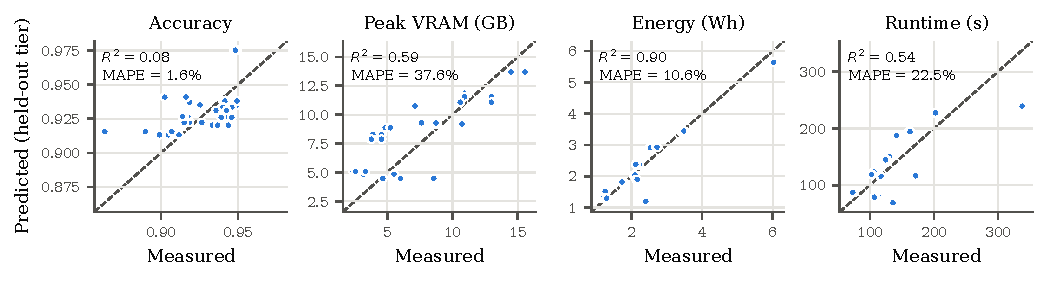
\includegraphics[width=\textwidth]{fig4_surrogate_loto.pdf}
\caption{Leave-one-tier-out predictions versus measurements for the 41 canonical
configurations. Each point is predicted by a model that never saw its backbone scale. The
dashed line is $y=x$.}
\label{fig:loto}
\end{figure*}

Energy is the one target that stays strong at an unseen scale: $R^2=0.897$ and MAPE 10.6\%
under leave-one-tier-out, so it is VALIDATED under every protocol. The other three targets
lose much of their accuracy once a scale tier is held out. Peak memory drops from
$R^2=0.929$ to 0.585, runtime from 0.982 to 0.544, and accuracy from 0.762 to 0.084.
Accuracy's MAPE stays at 1.6\% because the target barely varies, but at an unseen scale the
model is only modestly better than predicting the mean. The pass-grouped numbers should
therefore be read as interpolation results only. Seed grouping already removes much of their
optimism: accuracy $R^2$ falls from 0.762 to 0.390. Overall, the surrogate is
\textbf{PRELIMINARY}. It is accurate for energy and useful for shortlisting configurations
within the measured range. It is not validated for accuracy, memory or runtime at unseen
scales. % [src: paper/data/audit_numbers.json governing_status_recomputed]

The pass-grouped and leave-one-tier-out figures in the project's audit report were computed
on the uncollapsed 82-row frame for three targets. They differ from Table~\ref{tab:surrogate}
by at most 2.3 MAPE points (memory, leave-one-tier-out: 39.9\% vs.\ 37.6\%). The released
command-line tool uses those slightly wider audit bands. % [src: results/surrogate/cv_metrics.csv]

\subsection{RQ3: Decision-support scenarios}

Table~\ref{tab:scenarios} lists the outputs of the released tool for four constraint
settings. Each entry is the configuration recommended under the stated constraints and
profile, not the best configuration. All values in the table are predicted.

\begin{table*}[t]
\centering
\caption{Decision-support scenarios (\texttt{green-peft recommend}). All accuracy, memory,
energy and \COtwo{} values are surrogate \emph{predictions}; \COtwo{} is derived from predicted
energy. The VRAM budget is applied with a 10\% safety margin. Feasible = candidates passing
the sanity and constraint filters (of 70).}
\label{tab:scenarios}
\small
% [src: paper/data/table4_scenarios.csv; paper/data/scenarios_raw.json]
\resizebox{\textwidth}{!}{%
\begin{tabular}{@{}lllcccccll@{}}
\toprule
Scen. & Constraints, profile & Recommended & Feas. & Acc. & VRAM (GB) & Energy (Wh) & \COtwo{} (g) & Pareto & Scope / confidence \\
\midrule
A   & VRAM 16, acc.\ $\ge0.90$, balanced        & SmolLM2-1.7B + QLoRA     & 33 & 0.942 & 5.33 & 3.59 & 2.33 & yes & Interpolated scale / MEDIUM \\
A-M & as A, measured cells only                 & TinyLlama-1.1B + LoRA    & 12 & 0.940 & 8.91 & 1.74 & 1.13 & yes & Measured / HIGH \\
B   & VRAM 8, acc.\ $\ge0.90$, strict\_carbon   & SmolLM2-360M + LoRA      & 15 & 0.911 & 2.53 & 1.11 & 0.72 & yes & Out of range (0.36B) / LOW$^\dagger$ \\
C   & VRAM 16, acc.\ $\ge0.93$, high\_accuracy  & Phi-3-mini (3.8B) + QLoRA & 21 & 0.954 & 8.00 & 7.60 & 4.94 & yes & Out of range, unseen family / LOW$^\dagger$ \\
\bottomrule
\end{tabular}}
\par\smallskip\raggedright\footnotesize $^\dagger$Error bands are lower bounds: the surrogate
was never validated outside 0.5--3.0B. Highest-ranked measured alternative: B, Qwen2.5-0.5B +
LoRA (rank 3); C, Qwen2.5-3B + QLoRA (rank 2).
\end{table*}

\begin{figure}[t]
\centering
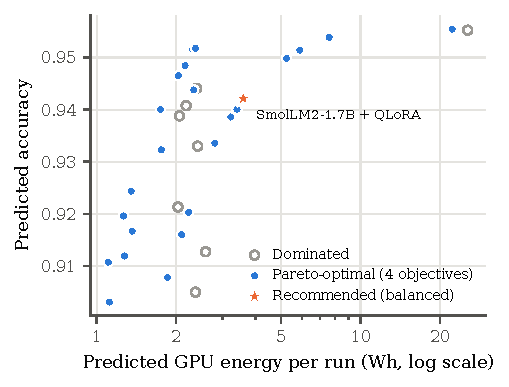
\includegraphics[width=\columnwidth]{fig5_pareto_scenarioA.pdf}
\caption{Scenario A: the 33 feasible candidates in predicted accuracy versus predicted energy
(log scale). The frontier is computed on four objectives (accuracy, memory, energy,
runtime), so some Pareto-optimal points look dominated in this two-dimensional projection.
All values are predictions.}
\label{fig:pareto}
\end{figure}

The scenarios show how scope labels change what a recommendation means. Under scenario A,
the balanced profile ranks an unmeasured 1.7B model first. It sits between measured scales,
so its confidence is MEDIUM. Restricting the search to measured cells (A-M) returns
TinyLlama-1.1B with LoRA. That candidate has a lower predicted energy (1.74 vs.\ 3.59\,Wh)
and a higher predicted memory (8.91 vs.\ 5.33\,GB), which reflects the weight that the
balanced profile places on memory. With an 8\,GB budget and the \texttt{strict\_carbon}
profile (B), the top candidate is a 0.36B model below the measured range. Its error band is
a lower bound, and the highest-ranked measured alternative is Qwen2.5-0.5B with LoRA. Under
\texttt{high\_accuracy} with an accuracy floor of 0.93 (C), the top candidate is an
out-of-range model from an unseen family. The runner-up, Qwen2.5-3B with QLoRA, is a
measured cell. % [src: paper/data/scenarios_raw.json]
In every scenario the recommended configuration lies on the Pareto frontier.
Fig.~\ref{fig:pareto} shows the frontier for scenario A.

\textbf{Recommendation validation.} The tool includes a back-test that re-predicts already
measured configurations. Those rows are in-sample: the back-test checks that the path from
candidate to features to model is correct, not that the surrogate generalises. No new
fine-tuning run has been recorded to test a recommendation out of sample. % [src: results/recommendation_validation.csv: all rows in_sample=True]

% =====================================================================================
\section{Discussion}

The study supports three conclusions within its scope. First, PEFT methods trade different
resources against each other: on this hardware, the method with the lowest memory was not the
method with the lowest energy or runtime. A single ``efficiency'' number would hide that,
which is why the decision layer keeps four objectives and leaves their weighting to the user.

Second, energy is the most predictable cost. A linear model on log energy, with features that
encode parameter count, bit width and trainable size, extrapolated to a held-out scale with
about 10\% error. The memory, runtime and accuracy models did not extrapolate as well. Four
scale tiers give little leverage for a cross-scale trend, and memory carries a systematic
measurement artifact.

Third, the measurement audit mattered more than the choice of model. Before the audit, the
pooled passes had made energy look unpredictable, and a method ranking computed on them
reflected the telemetry defect rather than the methods. Studies that report Green AI
metrics should check that power readings are physically plausible under load before using
them.

The decision layer is designed around those limits. Feasibility is decided by the
constraints, with headroom on the weakest prediction (memory). The GEI only orders options
that are already feasible, and every output carries its evidence scope. GreenPEFT is
therefore a shortlisting aid whose recommendations should be confirmed by running them. It is
not an autonomous selector.

% =====================================================================================
\section{Limitations}

\begin{itemize}
\item \textbf{Single GPU, single task.} All measurements come from one Tesla T4 and SST-2.
Nothing here establishes cross-hardware or cross-task behaviour.
\item \textbf{Four model scales} (0.5--3.0B). This is the binding constraint on every
extrapolation result. Predictions beyond 0.5--3.0B are unvalidated, and their error bands
are lower bounds.
\item \textbf{One valid energy pass.} Energy rests on a single trustworthy measurement per
configuration, with no telemetry replication.
\item \textbf{Fixed carbon intensity.} \COtwo{} uses one static factor (0.65\,kg/kWh). It is a
rescaling of energy and carries no independent uncertainty.
\item \textbf{Operational footprint only.} Embodied carbon, hardware lifetime, disposal and
e-waste were not measured.
\item \textbf{Provisional preference weights.} GEI profiles express project preferences, and
GEI values are relative to each candidate set.
\item \textbf{Single training budget.} All runs used 300 steps with fixed hyperparameters per
method, and no hyperparameter ablation (for example of LISA's sampling settings) was done.
\item \textbf{Incomplete method coverage across scales.} Not every method was measured at
every scale. Method-level summaries therefore mix backbones and should not be read as
rankings.
\end{itemize}

\textbf{Future work}, in priority order: (1) a second valid energy pass for the existing 41
configurations, checked against an independent power reading; (2) at least one measured
backbone outside 0.5--3.0B; (3) a second task; (4) a larger set of model scales; and
(5) additional GPU types. We do not expect more seeds per cell to help: across-seed variation
is small compared with the error from extrapolating across scales.

% =====================================================================================
\section{Conclusion}

GreenPEFT links measured PEFT cost to a pre-run surrogate and a constraint-aware decision
layer. On a controlled single-GPU SST-2 benchmark, the PEFT methods saved memory, energy and
time to different degrees. After a measurement audit removed an idle-floor telemetry pass,
energy could be predicted from pre-run metadata to about 10\% error at an unseen scale. The
remaining targets support interpolation and shortlisting but not confident extrapolation, so
the surrogate is rated preliminary. Every recommendation is labelled with its evidence scope
and should be treated as a candidate to measure, not a verdict.

% =====================================================================================
\section*{Reproducibility and Artifact Availability}

The harmonized dataset is available on Kaggle (DOI 10.34740/KAGGLE/DSV/20178095)
\cite{tanzil2026data}. The surrogate bundle is available on Hugging Face (GreenPEFT-v2,
revision 148b027, DOI 10.57967/hf/10690) \cite{tanzil2026model}. Code, raw per-run JSON and
the \texttt{green-peft} command-line tool (v0.3.0) are in the project repository
\cite{tanzil2026code}. \texttt{python reproduce.py} regenerates every derived artifact, and
\texttt{python reproduce.py --check} verifies them without writing. The figures, table inputs
and recomputed cross-validation in this paper are produced by
\texttt{paper/scripts/build\_paper\_assets.py} with scikit-learn 1.9.1. The surrogate was
validated with \texttt{GroupKFold} and \texttt{LeaveOneGroupOut} as described in the
Surrogate Model section.

\bibliographystyle{IEEEtran}
\bibliography{references}

\end{document}
